%%%%%%%%%%%%%%%%%%%%%%%%%%%%%%%%%%%%%%%%%%%%%%%%%%%%%%%%%%%%%%5
%% ITB Author: Ross Nolan
%%%%%%%%%%%%%%%%%%%%%%%%%%%%%%%%%%%%%%%%%%%%%%%%%%%%%%%%%%%%%%%5

\documentclass[12pt,ITBthesis]{report}

\usepackage{amsfonts}
\usepackage{amssymb,amsmath}
\usepackage{amsthm}
\usepackage{newlfont}
\usepackage{graphicx}
\usepackage{tabularx}
\usepackage{longtable}
\usepackage{lscape}
%\usepackage{rotating}
\usepackage{latexsym}
\usepackage{apacite}
\usepackage{natbib}
\usepackage{geometry}
\usepackage{fancyhdr}
\usepackage{xthesis}
\usepackage{xtocinc} %Include Table of Contents as the first entry in TOC
\usepackage{subfigure}
\usepackage{times}
\usepackage[hidelinks]{hyperref}

\bibpunct[, ]{(}{)}{;}{a}{,}{,}

\begin{document}

% Fuzz -------------------------------------------------------------------
\hfuzz2pt % Don't bother to report over-full boxes if over-edge is < 2pt
% Line spacing -----------------------------------------------------------

\newlength{\defbaselineskip}
\setlength{\defbaselineskip}{\baselineskip}
\newcommand{\setlinespacing}[1]%
           {\setlength{\baselineskip}{#1 \defbaselineskip}}
\newcommand{\doublespacing}{\setlength{\baselineskip}%
                           {2.0 \defbaselineskip}}
\newcommand{\singlespacing}{\setlength{\baselineskip}{\defbaselineskip}}
% MATH -------------------------------------------------------------------
\newcommand{\A}{{\cal A}}
\newcommand{\h}{{\cal H}}
\newcommand{\s}{{\cal S}}
\newcommand{\W}{{\cal W}}
\newcommand{\BH}{\mathbf B(\cal H)}
\newcommand{\KH}{\cal  K(\cal H)}
\newcommand{\Real}{\mathbb R}
\newcommand{\Complex}{\mathbb C}
\newcommand{\Field}{\mathbb F}
\newcommand{\RPlus}{[0,\infty)}
%
\newcommand{\norm}[1]{\left\Vert#1\right\Vert}
\newcommand{\essnorm}[1]{\norm{#1}_{\text{\rm\normalshape ess}}}
\newcommand{\abs}[1]{\left\vert#1\right\vert}
\newcommand{\set}[1]{\left\{#1\right\}}
\newcommand{\seq}[1]{\left<#1\right>}
\newcommand{\eps}{\varepsilon}
\newcommand{\To}{\longrightarrow}
\newcommand{\RE}{\operatorname{Re}}
\newcommand{\IM}{\operatorname{Im}}
\newcommand{\Poly}{{\cal{P}}(E)}
\newcommand{\EssD}{{\cal{D}}}
% THEOREMS ---------------------------------------------------------------
\theoremstyle{plain}
\newtheorem{thm}{Theorem}[section]
\newtheorem{cor}[thm]{Corollary}
\newtheorem{lem}[thm]{Lemma}
\newtheorem{prop}[thm]{Proposition}
%
\theoremstyle{definition}
\newtheorem{defn}{Definition}[section]
%
\theoremstyle{remark}
\newtheorem{rem}{Remark}[section]
%
\numberwithin{equation}{section}
\renewcommand{\theequation}{\thesection.\arabic{equation}}
%%% ----------------------------------------------------------------------
\setlength{\tclineskip}{1.05\baselineskip}
%%% ----------------------------------------------------------------------
\makeatletter
\renewcommand\appendix{%
 \par
 \setcounter{chapter}{0}%
 \setcounter{section}{0}%
 \setcounter{subsection}{0}%
 \gdef\thesection{\@Alph\c@section}
 \gdef\@sect##1##2##3##4##5##6[##7]##8{%
  \refstepcounter{##1}%
  \protected@edef\@svsec{\@seccntformat{##1}\relax}%
  \begingroup
    \hspace{-\parindent}##6\appendixname~ {%
    \@hangfrom{\hskip ##3 \relax\@svsec}\par%
    \hspace{-\parindent}\interlinepenalty \@M ##8 \@@par}%
  \endgroup
  \csname ##1mark\endcsname{##7}%
  \addcontentsline{toc}{##1}{\protect\numberline{\csname the##1\endcsname}##7}%
  \@xsect{##5}%
 }%
}%
\makeatother

\setlength{\parskip}{1ex plus 0.5ex minus 0.2ex}

\title{Test driven development of a game built with Unity and C\#}

\author{Ross Nolan }

\university{Institute of Technology Blanchardstown }

\dept{School of Informatics and Engineering }

\address{Dublin, Ireland }

\supervisor{Dr. Matt Smith }

\submitdate{19 April 2018 }

\degree{M.Sc. in Computing }


\setcounter{page}{1} \beforepreface

{ \typeout{Abbreviations}
% Thesis Abbreviation ------------------------------------------------------

\prefacesection{Abbreviations}

\begin{longtable}{p{90pt}l}
\hline MVC      & Model View Controller \\
\hline TDD      & Test Driven Development \\
\hline
\end{longtable}

% ----------------------------------------------------------------------
 %write your list of abbreviations in a file called abbreviations.tex
}

% ------------------------------------------------------------------------
\afterpreface
\def\baselinestretch{1}
\setlinespacing{1.66}
% ------------------------------------------------------------------------

\pagestyle{fancy}
\renewcommand{\chaptermark}[1]%
{\markboth{\MakeUppercase{\thechapter.\ #1}}{}}
\renewcommand{\sectionmark}[1]%
{\markright{\MakeUppercase{\thesection.\ #1}}}
\renewcommand{\headrulewidth}{0.5pt}
\renewcommand{\footrulewidth}{0pt}
\newcommand{\helv}
{%
\fontfamily{bch}\fontseries{b}\fontsize{9}{11}\selectfont} \fancyhf{} \fancyhead[LE,RO]{\helv \thepage}
\fancyhead[LO]{\helv \rightmark} \fancyhead[RE]{\helv \leftmark}

% ------------------------------------------------------------------------
\setlinespacing{1.0}

\setlinespacing{1.1}

\chapter{Introduction and Background} \label{sec:introduction}

\section{The Game}

The game is a puzzle adventure. It uses programming logic to solve the puzzles presented. 

\subsection{Serious Games}


\section{Architectural Patterns}
Describes how the MVC relates to my project

\subsection{MVC}

Using MVC architectural patterns are a common choice for games development. It is favoured for its modular
 approach. The separation of the model view controller interfaces allow me to build on each module without disturbing the other. When i need to expand on the development of the model class, i will be able to do with ease. There will be minimal, if any, disturbance's to the rest of the program. When the changes are made from the model class, those changes can be displayed to the user interface.

The LevelModel class represents the structure of data that holds the attributes of a level design. The LevelView class will display the attributes to the user interface . The LevelController class is used to exchange data between the two objects. In the case of this project, the LevelController will also manage the Input controller. 


	
\subsubsection{Model}

\subsubsection{View}

\subsubsection{Controller}



\subsection{Singleton}

\subsubsection{Don't Destroy On Load}



\section{Test Driven Development}

\subsection{Subsection header 1}

\newpage

\newpage

\section{Git Hub, Version Control}

\section{Games Development}

\subsection{Unity Engine}

level editor

reading file

NetHack ...

\begin{description}
	
 \item[C\#, Syntax, Refactoring:]
 
\end{description}







\chapter{Literature Review}


\section{Abstract}
Today our student are being labelled as digital natives. As this is the case, it leaves an area for more investigation. Computer programming is being brought into junior schools across the world. It's no longer a hobby for enthusiasts. The curriculum of computer science is evolving and the data flow of subjects is being changed regularly. Serious Games have been used for a number years to introduce different subjects. There is a case in Italy where they introduce workers to a restaurant through a Serious Game. It brings them through the restaurant and how to deal with customers through a text speech game. There is a multitude of Serious Games. This literature review explains in detail Serious Games in the genre of computer programming. These games are designed to teach novice programmer's the basics of computer programming and computer programming logic. With student understanding these basics, it gives them a stronger foundation for understanding programming concepts.

Index: Computer Science, Serious Games, Games Development

\section{Introduction}
As we progress more into the digital era we need to educate the natives in the latest trades. Computer science in some schools across the globe is being introduced as a subject with state exams. TAMPA Preparatory School in Florida, America, has introduced Robot C, C programming, and Swift iOS app development to go along with engineering and robotics \cite{thompson2017coding}. Coder Dojo is another example of pro-programming. Its an out of school club, young and old people can join. They hold coding events on weekends where they teach the student how to code. There are also other courses that teach computing through a single context, digital storytelling workshops, and robotics camps. Computer Science is becoming a more widespread field. A majority of everything that is delivered to us has Computer Science embedded into it, from the machines that make your clothes to your toothbrush. Our daily life revolves around the Internet of the things, whether it's in front of us or related to it in some way. As this is the case, the education of programming languages and programming logic is important for these students. Serious games or educational games is a good way to introduce novice programmer to the understanding of programming comprehension, see: Related Work section.
The reason for this literature review is to answers question's on how to develop the research project. The following questions need to be answered.

\begin{description}
	\item[$\bullet$] With today’s student’s, are digital games a good platform for education?
	\item[$\bullet$] Considering Serious Games about programming and programming logic. Who uses them as tools for learning? What was the general approach for their use? What age group is using them? Are people using them for past times or for learning?
	\item[$\bullet$] One of the issue's educational digital games have in a learning environment is that they may not address the subject in full. How can this project be delivered so that it addresses the depth of that subject?
\end{description}


\section{Related Work}
When teaching programming, one of the concepts that need’s to be grasped is programming logic. If a programming language is taught with the logic in an introductory computing class, it tends to ”distract from the core issue of algorithmic problem solving” (Shackelford and LeBlanc 1997). Programming Comprehension is when the student understands what the program is doing (Gugerty and Olson 1986). The author of (Lu and Fletcher 2009) suggest that computational thinking is required to prepare students for programming courses §3. New students to a programming module may have problems because they lack the programming comprehension, even if they can remember the syntax. Through the use of games, as a complement to the standard teaching curriculum, teachers found that the lessons are more absorbed than with a stand-alone lesson (Carrington, Baker, and van der Hoek 2005).

Educational games or Serious Games are designed so as not to intimidate the user who is unfamiliar with a specific subject. Serious Games are designed for a specific purpose (Deterding, Dixon, Khaled, and Nacke 2011). In the case of games based on programming or programming logic, they are useful to a student who does not understand the concept of ”loops or iteration”. There are a number of games that exist that aim to deliver the comprehension before the syntax.

\section{RobotOn!}
RobotOn!(Miljanovic and Bradbury 2016) was designed for first year Computer Science students learning C++. The user's average age was between 18-20 years of age. It was built with the cross-platform game engine Unity using C\# as its scripting language. It is a game that helps the student understand programming comprehension(Miljanovic and Bradbury 2016). The game has a number of different tools and comprehension tasks that are based on simple programming concepts. The tasks are given to teach control flow, code behavior, variable purpose and data flow. As they progress through the stages, their progress is saved to log files. Once they have completed the game, the students will have a basic understanding of programming comprehension.(Miljanovic and Bradbury 2016).

The author's methods were to evaluate the student's experiences with a number of questions. Is the game playable for undergraduate students? Do the students enjoy the game? Does RobotOn! teach C++ comprehension sufficiently? These are all relevant questions toward the future development of educational or serious games. Answers to questions like this will help designers in future to create a more directed approach to building serious games. Having a keener sense to what a student needs, is the underlying answer on how to develop these games. Unfortunately, there were no results for this particular study.

\section{Alice2}
Alice2 (Kelleher, Cosgrove, Culyba, Forlines, Pratt, and Pausch 2002) is designed to help students understand programming through building a 3D world with a drag and drop approach. With this design, it prevents syntax error's giving the user more confidence to experiment.The author believes there are 3 main tasks a new user might find difficult. 1) Finding a structured solution to a problem. 2) Express the solution in a syntax. 3) Understand the behavior of the program. In a user test of Alice1, they found that typing the syntax was a dominant problem(Pierce, Audia, Burnette, Christiansen, Cosgrove, Conway, Hinckley, Monkaitis, Patten, Shochet, et al. 1997).
In Alice2, the interface consists of a scene window, an object tree, the object details area, the animation editing area and the behaviors area. The user is able to drag and drop commands into animations giving it a result of the animation moving. One of the observations made during the study was that the students would often look through an object tree for ideas on what to build. This leaves the impression that worrying of correct syntax was not there. Alice2 capable of building programs to the size of 3000 lines(Kelleher, Cosgrove, Culyba, Forlines, Pratt, and Pausch 2002). Alice2 gives the user the opportunity to explore conditionals, count loops, while loops, variables, parameters, and procedures. It also implements a simple form of parallel programming and programming constructs found in Java and C++.

\section{Lightbot!}
The author of Lightbot states, "It(programming) is more about the process with which we come to a solution and think algorithmically about how to solve a problem.". Lightbot is a programming puzzle game. The solution to the puzzles is in direct correlation with programming concepts. LightBot puzzle game is a drag and drop game. You drop the tile commands into an instruction box, telling a character on the screen what do. The objective is to light up all the ground blue tile’s in each level. Each of the command tiles represents a different move, for example, move forward one space or light up the tile the character is standing on. The author states the game is broken up into two sections, Programming Practices, and Control-Flow. Programming practices are - Planning, Programming, Testing then Debugging. ControlFlow is - Sequence Instructions, Procedures, and Loops.

\subsection{Computational thinking(LightBot)}
In Computational thinking in Education(Gouws, Bradshaw, and Wentworth 2013), the authors address the problem of identifying, evaluating and incorporating computational thinking into education. They use a framework to assess computational thinking in the game LightBot. Their author named the framework, Computational Thinking Framework(CTF). It designed to work for a range of applications.The CTF is pictured in Figured 1.


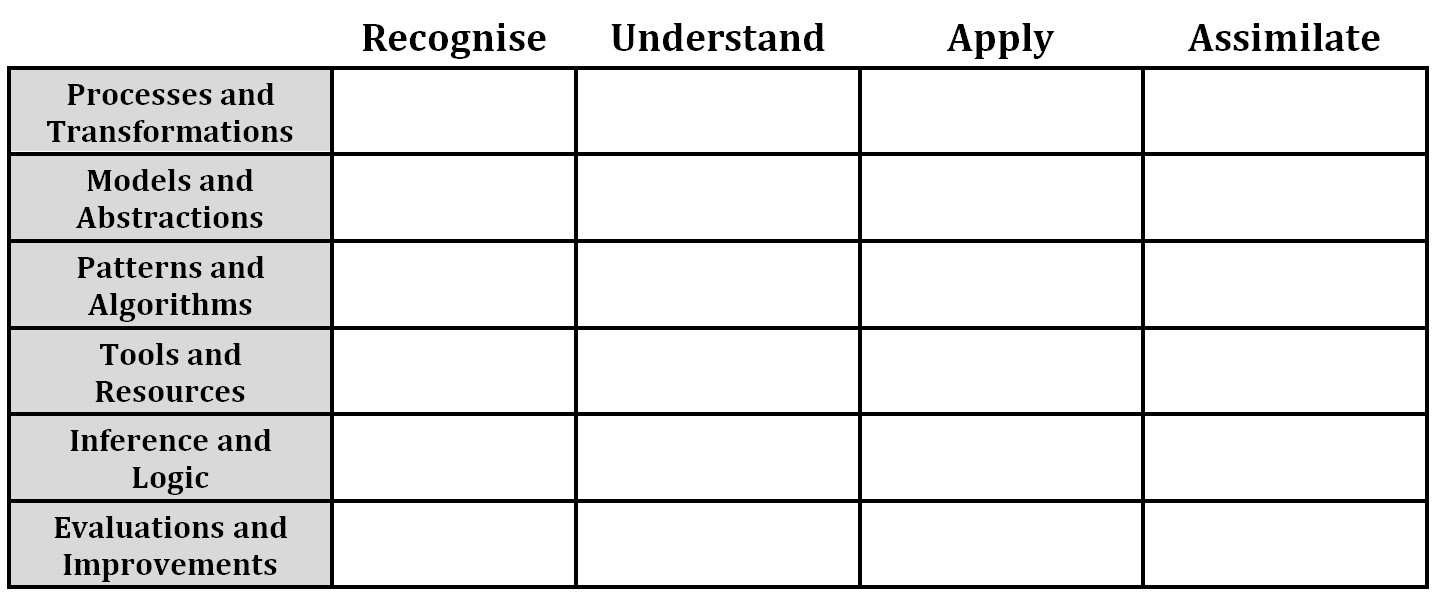
\includegraphics[scale=0.35]{CTFModel.png}

Figure 1: CTF model

The vertical axis is broken down into 6 distinct areas.

\begin{description}
	\item[$\bullet$] Process and Transformations
	\item[$\bullet$] Models and Abstractions
	\item[$\bullet$] Patterns and Algorithms
	\item[$\bullet$] Tools and Resources
	\item[$\bullet$] Inference and Logic
	\item[$\bullet$] Evaluations and Improvements	
\end{description}

The horizontal axis is broken down into what the authors call 4 levels.

\begin{description}
	\item[$\bullet$] Recognize
	\item[$\bullet$] Understand
	\item[$\bullet$] Apply
	\item[$\bullet$] Assimilate	
\end{description}

\subsection{The vertical axis}

\subsubsection{Process and Transformations}
Computational exercises circle around Processes and Transformation(Hu 2011). The student can also be introduced to activities of input, output and parallel processes(Hu 2011). This section is breaking down a problem into multiple steps and then solving in a logical manner.

\subsubsection{Models and Abstractions}
The student needs to think abstractly to create elegant solutions to such problems as data storage and manipulation(Hu 2011). Models can reinforce the comprehension of abstraction(Hu 2011).This section is how to represent a problem and solution(Gouws, Bradshaw, and Wentworth 2013).

\subsubsection{Patterns and Algorithms}
The author says that the likes of loops and iteration would all be representative of patterns in computer science(Hu 2011). If a student is able to recognize a pattern this will help them solve a problem(Hu 2011). This section is the ability to recognize patterns in a problem(Hu 2011).

\subsubsection{Tools and Resources}
The author views programming as tools for students. The student's way of thinking with programming is using tools to help solve a problem.A student selecting an appropriate tool to solve a problem is an accomplished programmer(Hu 2011). This section represents the availability of tools used to solve a problem(Hu 2011).

\subsubsection{Inference and Logic}
The student use of logic is important to solve computational problems. This section represents the logical skills used to solve a problem.

\subsubsection{Evaluations and Improvements}
The level a student can locate and break down a problem for an error. The level of understanding of why the error occurred.This section represents debugging and performance.

\subsection{The Horizontal Axis}

\subsubsection{Recognize}
At the recognized level this represents the student's ability to recognize and remember computational problems.

\subsubsection{Understand}
This level correlates to the student's comprehension of the computational problem.

\subsubsection{Apply}
This level relates to the student's ability to apply a solution to the given problem.

\subsubsection{Assimilate}
This level will measure the student ability to use the tools given in full. How to use smaller solutions with larger ones to solve a problem.

\subsection{LightBot Case Study}
The authors used LightBot to collect a Computational Thinking Score. After studying all the different levels they, they were able to gather what type of skills were required to pass the level. They then filled out the CTF and score were assigned to each block. Scores ranging from 0-3 indicate whether a concept is complete or not, 0 being least and 3 being best. The scores are then aggregated and converted to a percentage. The results were as follows in Figure 2.

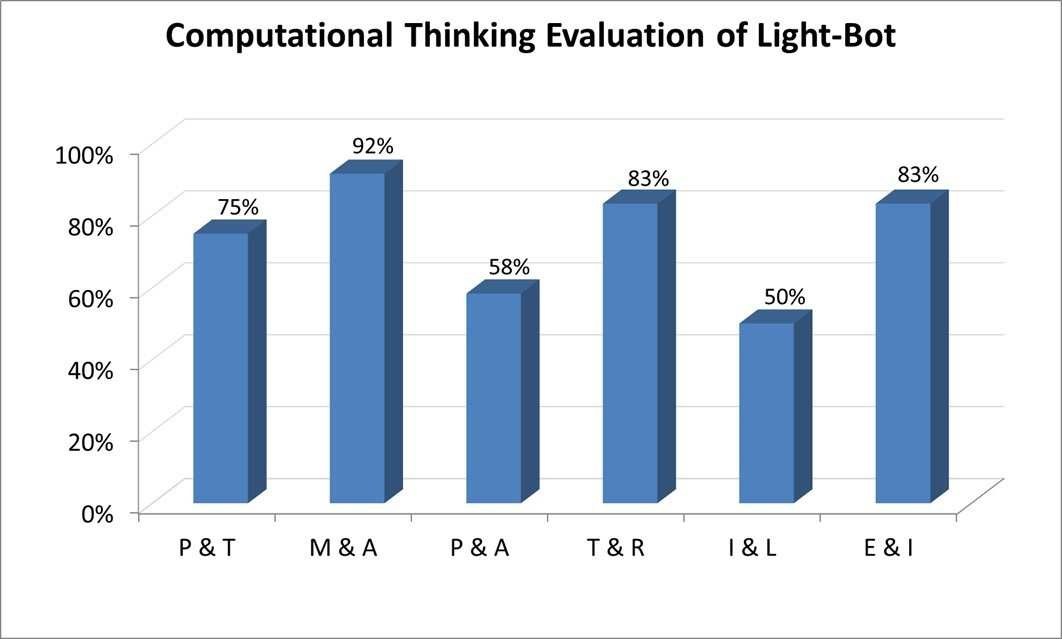
\includegraphics[scale=0.35]{resultsOfTest.png}

Figure 2: Results of Test

When developing a serious game a framework like this should be taken into account. The results show where an application could need to be improved, giving the designer a more focused idea on how to deliver the intended message.

\subsection{Conclusion}
In conclusion to this review, Serious Games, and my research project, Serious Games is an area continuing to grow as with the rest of the Computer Science sector. As there is more investigation into the subject, a more thorough model will develop to answer translations of lessons to games.
CTF has been used to evaluate project's to increase the level of usefulness towards understanding the computational thinking. After developing the Serious Game, it will use the CTF to gather a score. The game will be adjusted to gain scores where necessary.
The drag and drop system for input of code used in both Alice2 and Lightbot have a strong appeal to the user who is unfamiliar with syntax. As it is a strong approach to the novice to make them feel more confident in the complications of programming,  the game will be implementing this into the research project.

\section{section header 1}




\subsection{Subsection header 1}




\subsection{Subsection header 2}




\subsection{Subsection header 3}




\subsection{Subsection header 4}














































\section{Notes}

Faster performance, on game logic, not really a big deal,
but i other situations it is.

Why faster performance
Faster performances and possibly bad code vs normal performance and solid code(tested??).

CPU cycles

Design patterns , for and against, and why MVC

General thoughts on techniques picked up along the way
//commenting on exact places as i try to debug(tricks of the trade)

what is the point of a thesis
From my understanding, a thesis is another word for dissertation.  Both are names for a written report about the research that you have done as part of your academic requirements.

Naming Convention
From my own study and experience, when naming variables they need to make sense, and to follow up with where the logic is directed. Else, its hacky.

Dynamic Naming??Providers... For better automatic comments...

URL to Git Hub, nice layout page

return (lightable == 0); returning true this kul instead of just true

unreachable code in a true false situation, or any for that matter

Order of invoke

Show study of Serious games

MVC 

refactoring

theres a few extra lines of code, but the way it works, is it will go straight to the value instead of a loop, removing the need to go through all other values

TDD

Data Providers

check nethack

public static readonly( SquareTypep[] LightableTiles = new SquareType[3];)

Game Logic (Performance)
Performance Scripts (Job lists?)
Entity Systems.
Which lead into no if else loops(Nvidia Self driving cars, actualy ,but they were onto somthing)
which brings it back to performances scripts, but removes game logic, because game logic isnt the heavy,i think)

Variables at the start of a program, the public private, check runtime,when they run and what happens to them.

Trying to eliminate all loops,find out what happens in the background from direct search in array, to a loop array,
Do a statistics on Loop and direct grab (Unity Profiler)

Programming baggage? Debt? Design debt, when i hard code because of order(for example), and then i cant use it later.

annonymous methods

List Action...func 

set the model(Level Model){
	//Alll on the same page
	
}

To make assertions about collections, you should use CollectionAssert:

CollectionAssert.AreEqual(expected, actual);
List<T> doesn't override Equals, so if Assert.AreEqual just calls Equals, it will end up using reference equality.

CollectionAssert.AreEquivalent

Delegates....
Event handlers...

Level State -> mapSize 10 -> playerX playerY start position [1,1] -> starting conditions(starting state), (State after move etc)

Display window(eidtor behaviour??)

noun and verbs to methods

Method signitures

Further work

Website....

hot controll on mouse click, no other buttons to be pushed when mouse pushed down

mcv sittng on top of service layer

Try to prove the way i did the MVC instatiation is the beter or a good way to do it
Also, try to prove that the way i did the loop is more efficient.

Object pooling!

UX- 2 arguments for a situation, where , direct mode would display the input, north south example,
or where just the instruction list would display. The direct mode, not needing the text because the user just pushed the button, but the list because the user need to see the list. Being a minimal approach.

Further work.. Fix program commands


Why am i using the specific methods, why am i using MVC, why test driven development, unity etc.
Are these methods really capable of addressing the objectives?
The project has a dominant MVC architectural pattern.

My objectives are:
\begin{itemize}	
	\item To build a puzzle game that will teach basic programming logic.	
	\item To develop a test driven game, for the purpose of fully tested code free from bugs.	
	\item To maintain and research MVC and the befits of using the pattern in games development.	
	\item To test a mid to high level style of programming.	
	\item To increase written code efficiency with elegant solutions.	
	\item To refactor where possible.
\end{itemize}	


\subsection{Research In action}
How am i going to execute the research specifically when it comes to the order of things,
Am i going to write the code and then test.

I might want to gain an initial understanding through writing the code, then
construct the tests.

Try to address how im going to research each objective.

Objectives     ....     Methods

Make sure the objective are all handled by at least one methods


\section{Research Plan}

\subsection{Exploratory}
If MVC or test driven methods are used often in the industry

\subsection{Descriptive}
How many company are using these methods

\subsection{Explanatory}
Why are these methods used



\chapter{Design and Implementation}

The design of the software is an MVC architecture for the main game logic components. These components are broken into two sepereate systems. The two systems are Direct Mode and Programming Mode. I will explain each one seperatly, and then explain how i implemented them both as one system. 



\section{Direct Mode Design}

Direct mode is an MVC structure, the main underlying direct mode component structure will be model. The class organizing the display of any component the user needs to see or interact with in the UI, is the view.The Direct Mode controller will allow the Programming Mode controller to access any of the methods needed. 



\section{Direct Mode Implementation}


\section{Programming Mode Design}


\section{Programming Mode Implementation}
%\include{chapter4}
%\include{chapter5}
%\include{chapter6}
%\include{chapter7}
%\include{chapter8}

\setlinespacing{1.0}

\bibliographystyle{apacite}
\bibliography{References}

%%$\left( \appendix
%\chapter*{Appendices}
 %  \nonumchapter{Appendices}
%\newpage





\end{document}
% ------------------------------------------------------------------------
%%%      \setlength\LTleft{1pt}
